%%
%% Beuth Hochschule für Technik --  Abschlussarbeit
%%
%% Hauptdokument
%%
%% 
%%
%%%%%%%%%%%%%%%%%%%%%%%%%%%%%%%%%%%%%%%%%%%%%%%%%%%%%%%%%%%%%%%%%%%%%
\documentclass[11pt, a4paper,parskip=half]{report}
%% Übersetzen als Entwurf
%\usepackage[entwurf]{bhtThesis}
%% Übersetzen für die Abgabe
\usepackage[abgabe]{bhtThesis}
\typeout{Projekt Spyhole}

%\usepackage{float} %benutze ich für das richtige setzen der Bilder
\usepackage{blindtext}   %für Blindtext in Kapitel 2
\usepackage{listings}
\usepackage{color}
\lstset{ 
  literate={ö}{{\"o}}1
           {ä}{{\"a}}1
           {ü}{{\"u}}1
           {Ö}{{\"O}}1
           {Ä}{{\"A}}1
           {Ü}{{\"U}}1
           {ß}{{\ss}}1
}

%%\usepackage{hyperref}

\usepackage{trsym}
\usepackage{bytefield}
\definecolor{light-gray}{gray}{0.90} %Code Hintergrundfarbe

\usepackage{longtable}

%%
%% Pfad zu den Bildern
%%
\graphicspath{
  {pictures/},
  {einleitung/pictures},
  {kapitel1/pictures/},
  {kapitel2/pictures/},
  {kapitel3/pictures/},
  {kapitel4/pictures/},
  {kapitel5/pictures/}
}

% julians einstellungen
\definecolor{darkBHT}{rgb}{0,0.5882,0.5529}
\setlength{\parskip}{6pt} 
\setlength{\parindent}{0pt}

\definecolor{lightgray}{rgb}{.9,.9,.9}
\definecolor{darkgray}{rgb}{.4,.4,.4}
\definecolor{purple}{rgb}{0.65, 0.12, 0.82}

\lstdefinelanguage{JavaScript}{
  keywords={typeof, new, true, false, catch, function, return, null, catch, switch, var, if, in, while, do, else, case, break},
  keywordstyle=\color{blue}\bfseries,
  ndkeywords={class, export, boolean, throw, implements, import, this},
  ndkeywordstyle=\color{darkgray}\bfseries,
  identifierstyle=\color{black},
  sensitive=false,
  comment=[l]{//},
  morecomment=[s]{/*}{*/},
  commentstyle=\color{purple}\ttfamily,
  stringstyle=\color{red}\ttfamily,
  morestring=[b]',
  morestring=[b]"
}

%%\renewcommand{\baselinestretch}{1.05} 
\begin{document}
\pagestyle{fancy}


% \maketitle %Deckblatt


\begin{titlepage}
	\begin{center}
		\Large
		Beuth Hochschule für Technik Berlin
		\textcolor{darkBHT}{\rule{\textwidth}{0.2cm}} \\
		\vspace{2 cm}
		\Huge
		\textbf{Spyhole}
		\vspace{2 cm}
		
		\begin{figure}[htbp]
			\centering 
			
\includegraphics[width=9cm]{BHT-Logo-Basis.pdf}  
		\end{figure}
		
		\vspace{3cm}
		\Large
		Seminararbeit für die Lehrveranstaltung \\
		\begin{tabular}{lcl}
			Model Based Design & bei & Herr Flemming\\
		\end{tabular} 
		\\
		\vspace{0.8cm}
		Eingereicht am \\
		10. Juli 2013 %\today % Aktuelles Datum
		\vspace{0.8cm}
		
		Eingereicht von \\
		\begin{tabular}{ll}
			Matthias Hansert & s42\\
			Markus Perkowski & s42\\
			Björn Hepner & s798148\\
			Julian Zoellner & s798465\\
			Niklas Knauer & s798163\\
		\end{tabular}

	\end{center}
	\vfill
	\textcolor{darkBHT}{\rule{\textwidth}{0.2cm}}
	\vspace{1 cm}
	\normalsize
	
\end{titlepage}

%
% EOF
%

\tableofcontents %Inhaltsverzeichnis


\pagenumbering{arabic}
%%%%%%%%%%%%%%%%%%%%%%%%%%%%%%%%%%%%%%%%%%%%%%%%%%%%%%%%%%%%%%%
%% Die Kapitel der Arbeitw
%%
%% Beuth Hochschule für Technik 
%%
%% Einleitung 1
%%
%%

\chapter{Einleitung}
Der stetige technologische Fortschritt sorgt in allen Lebensbereichen für immer neue Erfindungen und Ideen. Eine der größten Entwicklungsbereiche für Privatanwender liegt im intelligenten Wohnen. Hierbei handelt es sich im Allgemeinen um technische Hilfsmittel, die einer Person oder einer Personengruppe das Leben erleichtert. Diese Entwicklung dieser Gerätewird durch leistungsfähige Hardware sowie die mächtigen Entwicklungswerkzeuge ermöglicht. Die geringen Kosten und die Umfangreiche Dokumentation im Internet machen es auch Privatanwendern möglich ihre eigenen Ideen zu verwirklichen.  
\par
Ein Teilbereich vom intelligenten Wohnen ist die Überwachung, in den sich auch dieses Projekt einordnen lässt. Mit dem Spyhole soll es möglich werden für Bewohner Kontrolle und Sicherheit über die Haupteingangstür zu bekommen. Die Idee ist, von überall und jederzeit durch den Torsion seiner Behausung gucken zu können. Weiterhin ist das ferngesteuerte Öffnen sowie das Abfragen der letzten Besucher eine erstrebenswerte Funktionalität. In Zeiten dauerhafter Vernetzung und der Smartphones steht es auch außer Frage, dass eine entsprechende Applikation für diese Systeme bereitgestellt werden muss. Es ist jedoch ebenso an Alternativsysteme zu denken, da es zur Projektvision gehört den Zugriff von überall zu ermöglichen. 
\par
Als Grundlage für dieses Projekt soll dabei Hardwareseitig das Rasberry Pi verwendet werden, worauf in Kapitel 2 eingegangen wird. In Kapitel 3 wird die Android App beschrieben und auf dessen Funktionalitäten eingegangen. Auf Deskop App wird in Kapitel 4 genauer eingegangen. Eine Zusammenfassung der Ergebnisse und eine Reflektion über den Projektverlauf können in Kapitel 5 nachvollzogen werden. 
 %Einleitung
%%quellen
%% http://www.raspbian.org/RaspbianDocumentation
%% http://www.raspberrypiguide.de
%% http://www.raspberrypi.org
%%
%% Beuth Hochschule für Technik --  
%%
%% Kapitel 2 - Raspberry Pi
%%
%%	
\chapter{Raspberry Pi}

\lstset{language=C,
				backgroundcolor=\color{light-gray},
				%frame=single,
				tabsize=2,
				%numbers=left,
				numbersep=5pt,
				%numberstyle=\color{light-gray},
				basicstyle=\ttfamily\color{black}\small,
				keywordstyle=\color{HKS51}\bfseries,
				commentstyle=\color{HKS13}\slshape,,
				identifierstyle=\color{blue},
				stringstyle =\color{orange}}
				
				
Das Raspberry Pi ist ein kreditkartengroßer Einplatinencomputer von der \textit{Raspberry Pi Foundation}\footnote{Stiftung und Wohltätigkeitsorganisation in Großbritannien} entwickelt wurde. Mithilfe seiner 700 MHz starken ARM-CPU kann er nahezu alles was auch normale Desktoprechner können.\\

Ziel der Entwicklung des Raspberry Pi ist das Interesse an dem Studium der Informatik und ähnliche Fachgebiete zu fordern, bzw. einen günstigen Computer zum Programmieren und Experimentieren anbieten zu können.\\

Durch die geringe Leistungsaufnahme, günstigen Preis und viele verschiedene Ausbau- und Personalisierungsmöglichkeiten können Raspberry Pi’s für verschiedene Zwecke eingesetzt werden. Unter anderem sind beliebte Projekte für den Haushalt Wetterstationen, Radiosender, Media Center, NAS, etc.

\newpage

%%%%%%%%%%%%%%%%%%%%%%%%%%%%%%%%%%%%%%%%%%%%%%%%%%%%%%%%%%%%%%%%%%%%%%
\section{Hardware}
%%-------------------------------------------------------------------
\subsection{Technische Spezifikationen}

\begin{figure}[h]
  \begin{center}		%width=\linewidth
    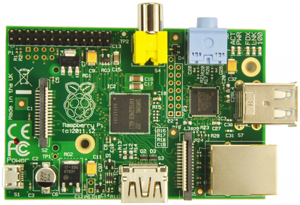
\includegraphics[scale=0.6]{raspberrypi-model-b.png}
  		  \caption{Raspberry Pi Model B}
     \label{raspPic}
  \end{center}
\end{figure}

\begin{longtable}{||l|l||}

\hline
Testfall & Fehler\\ \hline\hline
\endfirsthead
\hline
Testfall & Fehler \\ \hline\hline
\endhead

Größe & 85,60 x 53,98 x 17 mm\\ \hline
Soc & Broadcom BCM2835\\ \hline
CPU & ARM1176JZF-S(700MHz)\\ \hline
GPU & Broadcom VideoCore IV \\ \hline
SDRAM & 512MB\\ \hline
USB 2.0 & 2\\ \hline
Videoausgabe & HDMI \& S-Video\\ \hline
Tonausgabe & 3,5mm Klinkenstecker \& HDMI\\ \hline
Speicher & SD(SDHC/SDXC)/MMC/SDIO Kartenleser bis 128GB\\ \hline
Netzwerk & 10/100 MBit Ethernet\\ \hline
Schnittstellen & 17 GPIO-Pins, SPI, 21C, UART\\ \hline
Stromversorgung & 5V Micro-USB Anschluss\\ \hline

\end{longtable}
\footnote{http://www.raspberrypiguide.de; http://www.raspberrypi.org; 15.01.2014}


\newpage

%%-------------------------------------------------------------------
\subsection{Kamera}

\begin{figure}[h]
  \begin{center}		%width=\linewidth
    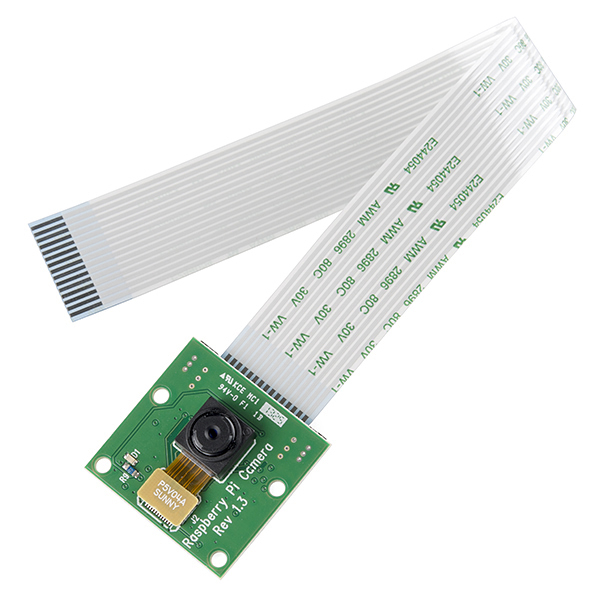
\includegraphics[scale=0.3]{camera.jpg}
  		  \caption{Raspberry Kamera}
     \label{raspCam}
  \end{center}
\end{figure}


\begin{longtable}{||l|l||}

\hline
Testfall & Fehler\\ \hline\hline
\endfirsthead
\hline
Testfall & Fehler \\ \hline\hline
\endhead

Größe & 20 x 24 mm\\ \hline
Sensor & OmniVision OV5647 (5MP)\\ \hline
Auflösung & 2592 x 1944\\ \hline
Video & 1080p \@ 30fps \\ \hline
Anschluss & 15-Pin Flachbandkabel\\ \hline

\end{longtable}


%%%%%%%%%%%%%%%%%%%%%%%%%%%%%%%%%%%%%%%%%%%%%%%%%%%%%%%%%%%%%%%%%%%%%%
\section{Software und Einstellungen}

%%-------------------------------------------------------------------
\subsection{Betriebssystem}
Für das Raspberry Pi worden mehrere Open Source Betriebssysteme programmiert. Alle basieren auf verschiedene Linux Distributionen(u.a. OpenSUSE, Fedora, FreeBSD, Debian). Je nach Bedarf kann sich jeder Nutzer für eine Distribution entscheidend, eins des beliebtestens Raspbian, basierend auf Debian, was auch in diesem Projekt benutzt wird. Raspbian inkludiert alle Grundprogramme und -Utilities dass mit vielen verschiedenen Packages kompatibel sind. Dieser Betriebssystem hat sich im laufe der Zeit als sehr stabil bewiesen.\\

Es gibt auch die Möglichkeit Windows auf das Raspberry Pi zu installieren, obwohl Nutzer davon abgeraten werden. Das Windows Betriebssystem benötigt zu viele Ressourcen und läuft sehr langsam und instabil auf das Raspberry Pi.\\

Andere Distributionen sind Gebrauchorientiert aufgestellt, wie zum Beispiel für Media Center das beliebte XBMC (OpenELEC, Raspbmc, XBian). Weiterhin gibt es auch Androidsysteme die auf das Raspberry Pi portiert worden sind.
\footnote{http://www.raspbian.org; 15.01.2014}


%%-------------------------------------------------------------------
\subsection{LAMP Webserver}
LAMP steht für Linux Apache MySQL PHP Webserver. Auf das Raspberry Pi wurde ein LAMP Server installiert um die Desktop/Mobil Applikation mit dem Pi zu verbinden und Informationen Austauschen. Durch die Einstellung eines DNS kann auf das Videostreams sowie auf die MySQL Datenbank zugegriffen werden. Damit \textit{http} oder \textit{ssh} Anfragen  an das Server im Raspberry Pi ankommen, müssen Ports für die Verbindung zur Verfügung gestellt werden. Im diesen Fall muss jeweils ein Port für die SSH-Verbindung, den Videostream und die Datenbankzugriffe freigegeben werden.\\

Um das LAMP Webserver zu installieren werden folgende Kommandos mit Administratorrechte ausgeführt:\\
\begin{lstlisting}
apt-get install apache2
apt-get install mysql-server
sudo apt-get install php5
sudo apt-get install php5-mysql
\end{lstlisting}

%%-------------------------------------------------------------------
\subsection{SSH Zugriff}
Damit das Team gleichzeitig auf das Raspberry Pi arbeiten konnte wurde auf das System eine SSH-Verbindung eingestellt. So wurden auch Entwicklungskosten gespart, weil nicht jeder Teammitglied ein System benötigte.\\

Um das Raspberry Pi per Fernzugriff zu betreiben ist es nötig eine \textit{Secure Shell} Verbindung aufzubauen. Durch die Verfügung einer SSH-Verbindung können Updates, Support und Wartungsarbeiten per Fernzugriff auf das System ausgeübt werden, dieses spart kosten für den Kunden sowie für den Support.

Als Sicherheitsmaßnahmen wurde der Standardport für SSH-Verbindungen (Port 22) auf ein anderen Port geändert und eine Public Key Authentifizierung implementiert. Um den Port für die SSH-Verbindung zu ändern, muss in der Datei \textit{/etc/ssh/sshd\_config} der Wert \textit{\#Port} auf den gewünschten Wert gesetzt werden. Danach muss das Dienst neu gestartet werden und somit ist der neue Port eingestellt.\\

Die Public Key Authentifizierung erfolgt indem der Benutzer ein privaten und einen öffentlichen Schlüssel erstellt. Der private Schlüssel wird am Client gespeichert und der öffentlicher Schlüssel am Server. Mit dem Befehl

\begin{lstlisting}
ssh-keygen -t dsa
\end{lstlisting}

werden die Schlüsseln generiert. Hier muss der Benutzer ein Passwort eingeben, mit dem sich er am Server anmelden wird. In der Regel heißen beider Schlüssel \textit{id\_das} und \textit{id\_das.pub}. Der private Schlüssel muss an das Client bekannt gemacht werden, indem man in der \textit{/ssh2/identification} Datei die Zeile 

\begin{lstlisting}
idkey id_dsa
\end{lstlisting}

bearbeitet oder einbaut. Der Inhalt des öffentlichen Schlüssels muss in der Datei \textit{/ssh/authorized\_keys} hinzugefügt werden.

\begin{lstlisting}
cat new_key.pub >> .ssh/authorized_keys
\end{lstlisting}

Jetzt ist der Client und der Server so konfiguriert, dass nur Rechner mit dem privaten Schlüssel Zugriff auf den Server haben über den konfigurierten Port.
Eine SSH-Verbindung wird mit folgendermaßen aufgebaut:
\begin{lstlisting}
ssh -p XXXX benutzer@serverAdresse
\end{lstlisting}

%%-------------------------------------------------------------------
\subsection{DNS}
Um das Raspberry Pi über das lokale Netz erreichbar zu machen, wurde erstmal ein Webserver aufgebaut. Um jetzt das System überall über das Internet erreichbar ist, muss eine Domain reserviert werden. Somit kann ein Benutzer Zugriffe auf die Datenbank, sowie auf das Videostream aus jedem Rechner oder Android Mobilgerät weltweit ausüben. Der Dienst ``no ip'' bietet solche Dienstleistung kostenlos an. Für dieses Projekt wurde die Adresse \textit{spyhole.no-ip.biz} eingestellt und durch die Freigabe und Weiterleitung von Ports können die programmierten Applikationen auf das Raspberry Pi zugreifen.\\

Da dieses Projekt im eine privaten Haushalt verwendet wird, besitzt in der Regel der Benutzer keine feste IP Adresse. Deswegen muss die IP Adresse hinter des DNS zyklisch geprüft werden. Der Dienst ``no ip'' stellt ein Programm zur Verfügung, das sich um die Überprüfung der Gültigkeit der IP Adresse kümmert. Das Programm muss dann mit den Kommandos

\begin{lstlisting}
make
make install
\end{lstlisting}

installiert werden. Während der Installation wird von den Benutzer das Login, Passwort und die Aktualisierungszeit verlangt. Danach wird der Dienst mit

\begin{lstlisting}
/usr/local/bin/noip2
\end{lstlisting}

gestartet. Der Dienst läuft bis das System runter gefahren wird. Daher ist es ratsam der Dienst im \textit{/etc/init.d} einzutragen.

%%%%%%%%%%%%%%%%%%%%%%%%%%%%%%%%%%%%%%%%%%%%%%%%%%%%%%%%%%%%%%%%%%%%%%
\subsection{Datenbanken}
Hier wird über die Datenbank und der Aufbau der Tabellen beschrieben. Als Datenbank benutzen wir MySQL-Server zur Speicherung der Daten. Zur Verwaltung der Daten in der Datenbank verwenden wir das Tool \texttt{phpMyAdmin}.

\subsubsection{Was ist SQL ?}
SQL ist einer der verbreitetsten Standards, um eine Kommunikation zwischen Server und Client mit Datenbanken zu ermöglichen. Mit SQL ist es möglich, Daten aus einer Datenbank zu selektieren, einzutragen, zu aktualisieren und zu löschen. Auch besteht die Möglichkeit mit Hilfe der SQL Tabellen in einer Datenbank zu erstellen, zu modifizieren oder zu löschen. Integriert ist ebenfalls eine Zugriffsverwaltung auf die Tabellen. 

Das Schema der Datenbank legt fest, welche Daten in einer Datenbank in welcher Form gespeichert werden können und welche Beziehungen zwischen den Daten bestehen. Insbesondere bei relationalen Datenbanken legt das Schema die Tabellen und deren Attribute sowie zur Sicherstellung der Konsistenz die Integritätsbedingungen fest. Dabei wird auch speziell der Primärschlüssel bzw. die Eindeutigkeitsbedingungen festgelegt.

\subsubsection{Was ist phpMyAdmin ?}
\texttt{phpMyAdmin} ist ein freies praktisches PHP-Tool zur Verwaltung von MySQL-Datenbanken. Das Tool bietet die Möglichkeit über HTTP mit einem Browser in MySQL neue Datenbanken zu erstellen bzw. zu löschen. Des Weiteren erlaubt das Tool die Erstellung, Löschung und Veränderung von Tabellen und Datensätzen. Auch die Verwaltung von Schlüssel-Attributen ist implementiert. Eine Anwendungsmöglichkeit des Tools \texttt{phpMyAdmin} ist die SQL-Statements direkt auszuführen und somit eine ausführliche grafische Abfrage der vorhandenen Daten in Form von Tabellen darzustellen. Für die Bedienung des Tools sind kaum Kenntnisse in SQL erforderlich, da das Tool nach dem WYSIWYG\footnote{ist das Akronym für das Prinzip „\textbf{W}hat \textbf{Y}ou \textbf{S}ee \textbf{I}s \textbf{W}hat \textbf{Y}ou \textbf{G}et“ (deutsch „Was du siehst, ist was du bekommst.“).} - Prinzip arbeitet.

\subsubsection{Aufbau}
\lstset{language=SQL,
				backgroundcolor=\color{light-gray},
				%frame=single,
				tabsize=2,
				%numbers=left,
				numbersep=5pt,
				%numberstyle=\color{light-gray},
				basicstyle=\ttfamily\color{black}\small,
				keywordstyle=\color{HKS51}\bfseries,
				commentstyle=\color{HKS13}\slshape,,
				identifierstyle=\color{blue},
				stringstyle =\color{orange}}
				
Die Datenbank \texttt{db\_spyhole} besteht aus drei Tabellen (tb\_doorloggers, tb\_users und tb\_images). In der  Tabelle \texttt{tb\_doorloggers} werden die Aktivitäten an der Tür gespeichert \textbf{(?)}, in der Tabelle \texttt{tb\_users} sind die registierte Users gespeichert, und die Tabelle \texttt{tb\_images} dient zur Speicherung der Bilder \textbf{(welche Bilder? Kommt noch dazu}).  

Ich werde den Aufbau der drei Tabellen genauer beschreiben:
\begin{lstlisting}[caption={Aufbau der Datenbanktabellen},captionpos=b]
--
-- Tabellenstruktur für Tabelle `tb\_doorlogger`
--

CREATE TABLE IF NOT EXISTS `tb\_doorlogger` (
  `ID` int(8) NOT NULL AUTO\_INCREMENT,
  `U\_ID` int(8) NOT NULL,
  `date` datetime NOT NULL,
  PRIMARY KEY (`ID`)
) ENGINE=InnoDB DEFAULT CHARSET=utf8 COLLATE=utf8\_unicode\_ci AUTO\_INCREMENT=1 ;
-- --------------------------------------------------------

--
-- Tabellenstruktur für Tabelle `tb\_images`
--

CREATE TABLE IF NOT EXISTS `tb\_images` (
  `ID` int(8) NOT NULL AUTO\_INCREMENT,
  `dl\_ID` int(8) NOT NULL,
  `U\_ID` int(8) NOT NULL,
  `imgdata` longblob,
  `imgtype` varchar(32) COLLATE utf8\_unicode\_ci DEFAULT NULL,
  PRIMARY KEY (`ID`)
) ENGINE=InnoDB DEFAULT CHARSET=utf8 COLLATE=utf8\_unicode\_ci AUTO\_INCREMENT=1 ;

-- --------------------------------------------------------

--
-- Tabellenstruktur für Tabelle `tb\_user`
--

CREATE TABLE IF NOT EXISTS `tb\_user` (
  `ID` int(8) NOT NULL AUTO\_INCREMENT,
  `name` varchar(64) COLLATE utf8\_unicode\_ci NOT NULL,
  `firstname` varchar(64) COLLATE utf8\_unicode\_ci NOT NULL,
  `email` varchar(128) COLLATE utf8\_unicode\_ci NOT NULL,
  `user` varchar(16) COLLATE utf8\_unicode\_ci NOT NULL,
  `password` varchar(255) CHARACTER SET utf8 COLLATE utf8\_bin NOT NULL,
  `u\_timestamp` timestamp NOT NULL DEFAULT '0000-00-00 00:00:00' ON UPDATE CURRENT\_TIMESTAMP,
  PRIMARY KEY (`ID`)
) ENGINE=InnoDB DEFAULT CHARSET=utf8 COLLATE=utf8\_unicode\_ci AUTO\_INCREMENT=1 ;

\end{lstlisting}
Das Attribut „ID“ vom Typ „INT“ kann Werte von  -2147483648 bis 2147483647 erfassen. Die Attribute vom Typ „VARCHAR()“ können beliebige Zeichenkombinationen speichern. Die maximale Zeichenlänge ist dabei von der in der Klammer befindlichen Zahl abhängig. Der Befehl „NOT NULL“ in der Definition der Attribute bewirkt, dass die entsprechende Spalte mit Daten vorhanden sein muss, sobald ein neuer Datensatz angelegt wird. Anders sieht es aber beim Befehl „DEFAULT NULL“ aus, dass die entsprechende Spalte nicht zwingend mit Daten gefüllt werden muss und standardmäßig auf NULL gesetzt wird, wenn ein neuer Datensatz keine Daten enthält. Das Attribut „ID“ wird als Primärschlüssel (Befehl „PRIMARY KEY (`ID`)“ definiert und mit AUTO\_INCREMENT zusätzlich ausgestattet. Das hat die folgende Bedeutung, dass das Attribut „ID“ fortlaufend um eins erhöht wird, wenn ein neuer Datensatz hinzufügt wird. Ein Primärschlüssel dient der eindeutigen Identifizierung der einzelnen Zeilen in einer Tabelle. 

%%%%%%%%%%%%%%%%%%%%%%%%%%%%%%%%%%%%%%%%%%%%%%%%%%%%%%%%%%%%%%%%%%%%%%
\section{OpenCV}

Ist eine freie Programmbibliothek(unter BSD-Lizens) mit Algorithmen für Bildverarbeitung und maschinelles sehen. Es beinhaltet C/C++, Python und Java Interfaces und unterstützt Windows, Linux, Mac OS, iOS and Android. OpenCV wird sowohl im kommerziellen wie im privaten Bereich stark benutzt.

%%-------------------------------------------------------------------
\subsection{Gesichtserkennung}
Unter die vielen Möglichkeiten das OpenCV anbietet, ist für dieses Projekt die Funktionen der Gesichtserkennung relevant.\\

hier kommt noch text\\


%%%%%%%%%%%%%%%%%%%%%%%%%%%%%%%%%%%%%%%%%%%%%%%%%%%%%%%%%%%%%%%%%%%%%%
\section{MJPG Streamer}
hier kommt noch text\\


%%-------------------------------------------------------------------
\subsection{subsection}

hier kommt noch text\\
 %Raspberry Pi
%%
%% Beuth Hochschule für Technik --  
%%
%% Kapitel 3 - Android App
%%
%%	

\chapter{Android App}
\section{Android}
Das Betriebssystem ist komplett in der Sprache Java programmiert worden. Dabei handelt es sich um ein Open Source Betriebssystem, welches von der Firma Google entwickelt worden ist. Kern des Betriebssystems ist ein angepasster Linux-Kernel 2.6. 
\subsection{Struktur und Aufbau der App}

\begin{figure}[h]
  \begin{center}
    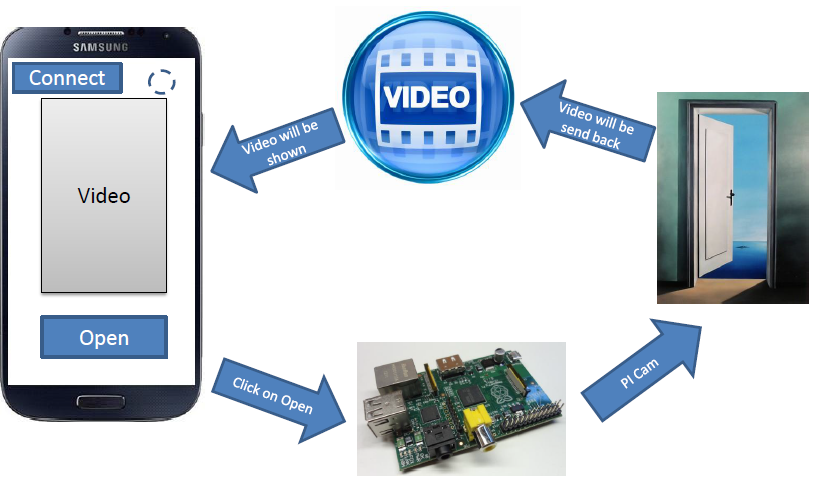
\includegraphics[scale=0.3]{process.png}
  		  \caption{Prozess der App}
     \label{fig.Prozess}
  \end{center}
\end{figure}
Sobald die Control-View geladen ist verbindet sich das mobile Endgerät mit dem Raspberry Pi. Nachdem die Verbindung aufgebaut wurde, kann der Benutzer der App die Schaltfläche \texttt{Open} betätigen. Nach der erfolgreicher Verbindung zum Server sendet dieser einen kontinuierlichen Live-Stream an das Endgerät. Wenn der Benutzter nun die Schaltfläche \texttt{Open} betätigt, wird ein Befehl zum Öffnen der Tür gesendet und ein GPIO angesteuert, der den Türöffner betätigt, um die Tür zu öffnen.

%%%%%%%%%%%%%%%%%%%%%%%%%%%%%%%%%%%%%%%%%%%%%%%%%%%%%%%%%%%%%%%%%%
\subsection{Anmelden des Users}
Um zu verhindern, dass nicht jede Person auf den Stream zugreifen kann, sollte aus Sicherheitsaspekten ein Login implementiert werden. Da aber unerwartete technische Probleme auftraten und diese in der Zeit nicht gelöst werden konnte wurde dieser Aspekt, erst einmal beiseite gestellt.
Jedoch wird im Folgenden auf die Vorgehensweise eingegangen, welche Technologien verwendet worden sind und wie der Login- und Registrierungsprozess ablaufen soll beschrieben.

\subsubsection{Registrierung}
\begin{figure}[h]
  \begin{center}
    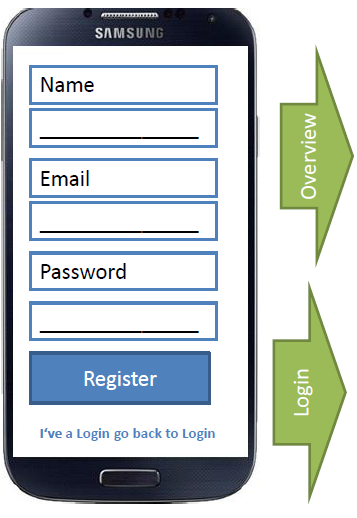
\includegraphics[scale=0.3]{register.png}
  		  \caption{Registrierung}
     \label{fig.Prozess}
  \end{center}
\end{figure}

Um sich überhaupt einloggen zu können muss sich der Benutzer beim aller ersten Mal  mit seinen Kontaktdaten registrieren. Dabei muss der Nutzer seine 
\begin{itemize}
	\item{E-Mail}
	\item{Nutzername}
	\item{Passwort}
\end{itemize}
eingeben.
Das Framework Android-SDK bietet es dem Nutzer an die grafische Oberfläche von der eigentlich Logik zu trennen. Die grafischen Oberflächen werden als Views betitelt. Die Views werden mithilfe von XML gestaltet.
\begin{lstlisting}[caption={Android - Button erstellen},captionpos=b]
<Button
       android:id="@+id/btnLinkToLoginScreen"
       android:layout_width="fill_parent"
       android:layout_height="wrap_content"
       android:layout_marginTop="40dip"
       android:background="@null"
       android:text="Already registred. Log Me In!"
       android:textColor="#21dbd4"
       android:textStyle="bold" />
\end{lstlisting}
In dem obigen Codebeispiel wird ein Button in der View erzeugt. Dabei wird dieser mit einer sog. ID versehen, um den Button über diese ID aus dem Quellcode ansprechen zu können. Mithilfe von \texttt{android:layout\_width} und \texttt{android:layout\_height} wird die Höhe und Breite des Buttons beschrieben. Die Option \texttt{fill\_parent} lässt den Button über die ganze Breite des Bildschirmes anzeigen, abhängig von der Auflösung des Endgerätes. Die Option \texttt{wrap\_content} lässt den Button nur so groß werden, dass alle Inhalte gut zu erkennen sind.
\\
Parallel zu der grafischen Gestaltung der Activity \texttt{Register.xml} wird die eigentliche Logik in Java-Klassen ausgelagert, um eine strikte Trennung von GUI und Fachlogik zu erreichen. Die Klasse \texttt{SignUp.java} ist diesem Fall die Klasse die sich auf das XML-File \texttt{Register.xml} referenziert. Um die einzelnen Objekte des Layouts ansprechen zu können, werden im ersten Schritt alle einzelnen Komponenten erzeugt und im Nachhinein mit der Funktion \texttt{Objekt.findViewByID.ObjektID} auf das jeweilige gerade erzeugte Objekt in der Java-Klasse referenziert.
%%%%%%%%%%%%%%%%%%%%%%%%%%%%%%%
%Code-Beispiel findVIew....
\begin{lstlisting}[caption={Objekt Erzeugung und Referenzierung},captionpos=b]
Button btnRegister;
btnRegister = (Button) findViewById(R.id.btnRegister);
\end{lstlisting}
%%%%%%%%%%%%%
Um überhaupt eine funktionierende Activity zu programmieren braucht man die Funktion \texttt{onCreat()}. In dieser Funktion wird all das ausgeführt was beim 
Starten der Activity passieren soll. Zum einen das Referenzieren auf die erzeugten Objekte und weitere Funktionsaufrufe.
%%%%%%%%%%%%%%%%%%%%%%%%%%%%%%%%
%%Was passiert nun in der Klasse Code und Beschreibung
%%%%%%%%%%%%%%%%%%%%%%%%%%%%%%%%
Um den neuen Nutzer zu registrieren wurden einige Funktionen in die Klasse \texttt{UserFunctions.java} ausgegliedert. Diese Funktion beinhaltet verschiedene Funktionen, die anderen Klassen wieder verwendet werden um einen Nutzer zu registrieren, zu prüfen ob er schon eingeloggt ist oder um ihn auszuloggen.
\begin{lstlisting}[caption={User Functions},captionpos=b]
    public JSONObject loginUser(String name, String password);
    public JSONObject registerUser(String name,  String password);
    public boolean isUserLoggedIn(Context context);
    public boolean logoutUser(Context context);
\end{lstlisting}
Die Funktion \texttt{registerUser(...)} bekommt zwei verschiedene String - Parameter um den neuen Nutzer in die Liste eintragen zu können. Zu einen den Name und zum anderen sein gewähltes Password.
\begin{lstlisting}[caption={registerUser(...)},captionpos=b]
// Building Parameters

   List<NameValuePair> params = new ArrayList<NameValuePair>();
   params.add(new BasicNameValuePair("tag", register_tag));
   params.add(new BasicNameValuePair("name", name));
   params.add(new BasicNameValuePair("password", password));

   // getting JSON Object
   JSONParser jsonParser = new JSONParser(registerURL, params,mContext);
   try {
         Thread.sleep(2000);
   } catch (InterruptedException e) {
         e.printStackTrace();
   }
   JSONObject json = jsonParser.getJSONFromUrl();
   Log.i("JSON4", json.toString());
   // return json
   return json;
\end{lstlisting}
Es wird eine Liste \texttt{params} mit dem Typ \texttt{NameValuePair} erzeugt. Anschließend werden die Übergabeparameter in die Liste eingefügt mit der Methode \texttt{params.add()}, plus einem Tag \texttt{register\_tag}.Im Nachhinein wird das JSON-Objekt zusammen gefügt und am Ende der Funktion das fertig erzeugte JSON-Objekt mit allen Inhalten zurück gegeben.
Das erzeugte JSON-Objekt wird per POST-Methode an den Server gesendet. Auf dem Server wird in der Index.php anhand des Tags erkannt, dass sich ein neuer Nutzer anmelden möchte dem entsprechend wird in einer Mehrfachauswahl (Switch-Case) ausgewertet und in einem weiteren PHP-Skript weiter bearbeitet. Schlussendlich werden die Daten in eine MySQL-Datenbank in die jeweiligen Spalten geschrieben. Das eingegebene Passwort wird  beim Eintragen in die Datenbank verschlüsselt, dass mögliche Hacker die das Password nicht auslesen können.
\\
Die weiteren Funktionen die in der Klasse enthalten sind, sprechen an für sich selbst und werden dem entsprechen nicht weiter erläutert.
\\
In der \texttt{SignUp.java} Klasse wird auf die response des Servers gewartet und bei einem erfolgreichen Registrieren wird der Nutzer der App weitergeleitet auf die Activity \texttt{OverView}.
\newpage

 
\subsubsection{Login}
\begin{figure}[h]
  \begin{center}
    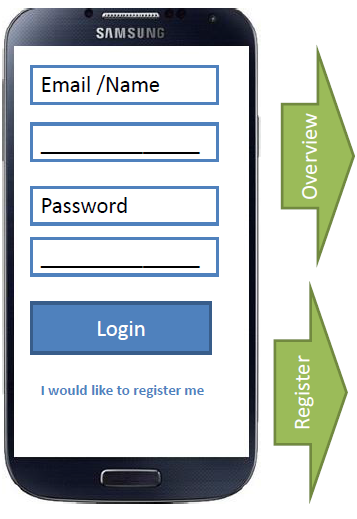
\includegraphics[scale=0.3]{login.png}
  		  \caption{Login}
     \label{fig.Prozess}
  \end{center}
\end{figure}

Beim Login verläuft der Vorgang wie bei der eben beschriebenen Registrierung, bloß in die andere Richtung. Dabei wird ein JSON-Objekt vom Server an das mobile Endgerät geschickt und in der App aufgeschlüsselt und interpretiert. Danach wird verglichen ob sich der Nutzer, der sich gerade einloggen möchte schon eingetragen ist, wenn ja wird er auf die nächste Activity weitergeleitet, ansonsten wird er zur Registrierung geführt und gebeten sich anzumelden.
\subsection{Control View}
\begin{figure}[h]
  \begin{center}
    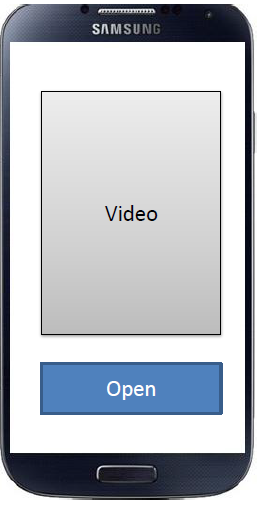
\includegraphics[scale=0.3]{controlcenter.png}
  		  \caption{Control View}
     \label{fig.Prozess}
  \end{center}
\end{figure}
Die Activity \texttt{ControlView} ist die Activity in der der Nutzer den Stream und die Öffnung der Tür vornehmen kann. Die Activity beinhaltet zwei Komponenten, zum einen die Webview in der der Stream mit der Gesichtserkennung dargestellt wird und zum anderen der \texttt{Open Butten}, mit dem das Signal zum Türöffnen gesendet wird.

\begin{lstlisting}[caption={Aufbau der Verbindung und darstellen des Streams},captionpos=b]
webView.getSettings().setJavaScriptEnabled(true);
//webView.setAlwaysDrawnWithCacheEnabled(true);
webView.setClickable(false);

// Create a progressbar
pDialog = new ProgressDialog(Control.this);
// Set progressbar title
pDialog.setTitle(" loading DigitalSpy");
// Set progressbar message
pDialog.setMessage("Buffering...");
pDialog.setIndeterminate(false);
pDialog.setCancelable(false);
// Show progressbar
pDialog.show();

// load and show the website
webView.loadUrl("http://spyhole.no-ip.biz/javascript_simple.html");

\end{lstlisting}
Sobald der Nutzer sich auf der Activity Control View befindet, beginnt die App sich mit dem Server zu verbinden und baut die Verbindung auf. Dabei war zu beachten das wir Javascript aktivieren, da wir den Stream mithilfe von Javaskript auf der Webseite darstellen. Um zu verhindern das der Nutzer die Tür öffnet bevor der Stream zu sehen ist, wurde eine Progressbar eingebaut, diese blockiert so lange die Activity so lange die Verbindung noch aufgebaut wird.

\subsection{Datenbank}
\begin{figure}[h]
  \begin{center}
    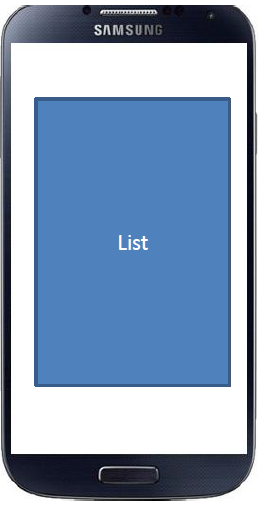
\includegraphics[scale=0.3]{database.png}
  		  \caption{Datenbank}
     \label{fig.Prozess}
  \end{center}
\end{figure}
Diese Activity stellt alle Öffnungen der Tür da. Die dargestellten Daten sind die selben die auch in der JavaFx App benutzt werden, sie werden aus der MySQl Datenbank ausgelesen in der Tabelle dargestellt.
Die Database Activity wird von \texttt{ListActivity} erweitert. \texttt{Database} beinhaltet zwei verschiedene Methoden zum einen die \texttt{getData()} und \texttt{fillList()}.  \texttt{getData()} stellt zuerst eine Verbindung zum MySQl- Server her und liest die Daten aus und speichert diese im Objekt \texttt{result} vom Typ ArrayList.\\
In der Methode \texttt{fillList()} wird dieses Objekt wieder verwendet und anhand der ausgelesenen Daten in die Liste in der App eingetragen. %Android App
%%
%% Beuth Hochschule für Technik --  
%%
%% Kapitel 3 - Desktop App
%%
%%	

\chapter{Desktop App}
Zu der Android App gibt es parallel eine App für den Desktop. Diese wurde mit JavaFX  programmiert. In den folgenden Kapiteln wird die ungefähre Programmierung der einzelnen Stages beschrieben.

\lstset{language=Java,
				backgroundcolor=\color{light-gray},
				%frame=single,
				tabsize=2,
				breaklines=true,
				%numbers=left,
				numbersep=5pt,
				%numberstyle=\color{light-gray},
				basicstyle=\ttfamily\color{black}\small,
				keywordstyle=\color{HKS51}\bfseries,
				commentstyle=\color{HKS13}\slshape,,
				identifierstyle=\color{blue},
				stringstyle =\color{orange}}
				
				
\section{Was ist JavaFX ?}
JavaFX ist eine Java-Spezifikation, die als Hauptkonkurrenten Adobe Flash und Microsoft Silverlight hat. Ein positiver Punkt ist der Lauffähigkeit auf diversen Geräten wie z.B. Mobilfunk, Desktop-Computern, Embedded Geräten und Blu-ray Geräten. Die Programmierung findet ganz normal wie in Java statt. Die dazu gehörigen Bibliotheken werden seit der Java SE Runtime 7 Update 6 automatisch mitinstalliert. Es ist unter anderem auf die Grafikprogrammierung ausgelegt. Dadurch lassen sich grafische Elemente schnell programmieren und mit CSS gestalten.
Ein sehr bekanntes Embedded Gerät, wofür es auch JavaFX gibt, ist das Raspberry PI. \cite{bib.jFXRaspPi}

\section{Struktur und Aufbau der App}
Es gibt insgesamt fünf verschiedene Stages in der App.
\begin{itemize}
	\item Login (siehe \ref{subsec.login})
	\item Registrierung (siehe \ref{subsec.registrierung})
	\item Control (siehe \ref{subsec.control})
	\item Datenbank (siehe \ref{subsec.datenbank})
	\item Foto (siehe \ref{subsec.foto})
\end{itemize}

In JavaFX ist ein Fenster ein Stage-Objekt. Diesem Stage-Objekt können mehrere anderer Objekte hinzugefügt werden. Bei diesen anderen Objekten kann es sich um Buttons, eine Tabelle, ein Textfeld usw. handeln.

\begin{figure}[h]
  \begin{center}
    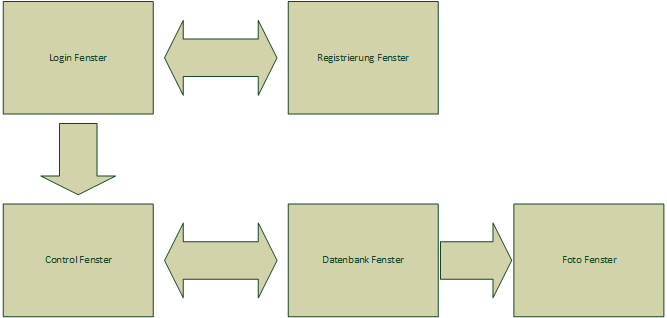
\includegraphics[scale=0.7]{MaskenDesktopVersion.png}
  		  \caption{Aufbau der App}
     \label{fig.MaskenDesktopVersion}
  \end{center}
\end{figure}\newpage

\subsection{Login}
\label{subsec.login}
Bei dem Login Fenster muss sich der Nutzer mit seinem Usernamen und Passwort, was in der Datenbank hinterlegt ist, anmelden. Ist einer der Felder nicht ausgefüllt oder das Passwort bzw. der User nicht korrekt, wird das mit einem \texttt{Label} als Message dargestellt. Über eine \texttt{CheckBox} kann der Benutzer sich sein Passwort in Klartext anzeigen oder verbergen lassen. Dies wurde so realisiert das ein \texttt{TextField} Objekt und ein \texttt{PasswordField} Objekt direkt übereinander gelegt wurden. Der Initialisierungszustand ist der, das das \texttt{PasswordField} sichtbar und das \texttt{TextField} unsichtbar ist. Mit der \texttt{CheckBox} wird das Ganze dann getoggelt.
\begin{lstlisting}[caption={Java Passwort-, Textfeld Un-, Sichtbar}\label{lst:reg.java.pw.txt},captionpos=b]
		pwTextField.managedProperty().bind(checkBox.selectedProperty());
		pwTextField.visibleProperty().bind(checkBox.selectedProperty());

		passwordField.managedProperty().bind(checkBox.selectedProperty().not());
		passwordField.visibleProperty().bind(checkBox.selectedProperty().not());
\end{lstlisting}
Damit das Eingegebene mit in dem anderen Feld erscheint, werden beide Felder bidirektional miteinander verbunden.
\begin{lstlisting}[caption={Java Passwort-, Textfeld bidirektional}\label{lst:reg.java.bidirektional},captionpos=b]
		pwTextField.textProperty().bindBidirectional(
						passwordField.textProperty());
\end{lstlisting}
\begin{figure}[h]
  \begin{center}
    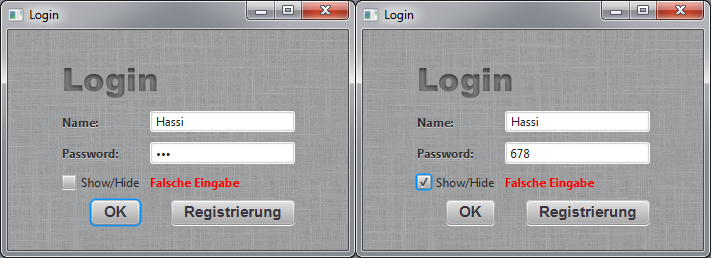
\includegraphics[scale=0.6]{loginStage.png}
  		  \caption{Login Fenster}
     \label{fig.loginFenster}
  \end{center}
\end{figure}

\subsection{Registrierung}
\label{subsec.registrierung}
Falls der Benutzer noch kein Konto in der Datenbanktabelle \texttt{tb\_Users} hat, hat er die Möglichkeit, sich über das Registrierungsfenster anzumelden. Softwareseitig wurde eine Überprüfung eingebaut, dass jedes Textfeld etwas beinhalten muss. Bei den Passwortfeldern wird überprüft, ob die beiden Passwörter, die eingegeben wurden, identisch sind. Wenn alle Überprüfungen korrekt sind, wird aus den Eingaben und einem SQL Befehl \texttt{NOW()} ein SQL-String gebaut und an die Datenbank geschickt. Falls die Überprüfung fehlgeschlagen ist, wird wie im  Login Fenster (s. \ref{subsec.login}) eine \texttt{Label} Message ausgegeben.
%%%%%%%%%%%%%%%%%%%%%%%%%%%%%%%%%%%%%%%%%%%%%%%%%%%%%%%%%%%%%%%%%%%%%%%%%%%
%referenz auf die DB wie sie aufgebaut ist ???
%%%%%%%%%%%%%%%%%%%%%%%%%%%%%%%%%%%%%%%%%%%%%%%%%%%%%%%%%%%%%%%%%%%%%%%%%%%
\begin{lstlisting}[caption={Java-SQL neuer Benutzer}\label{lst:reg.java.eintrag},captionpos=b]
	String SQL = "INSERT INTO tb_user VALUES (null,'"
									+ txtVorname.getText() + "', '"
									+ txtNachname.getText() + "', '"
									+ txtEmail.getText() + "', '"
									+ txtUserName.getText() + "', '"
									+ txtPw.getText() + "', NOW())";
\end{lstlisting}
Der folgende String zeigt die Darstellung, wie der obige String mit Nutzerdaten aussieht und an die Datenbank gesendet wird.
\begin{lstlisting}[caption={SQL Beispiel String}\label{lst:reg.sql.eintrag},captionpos=b]
	INSERT INTO tb_user VALUES (null,'Gernot', 'Hassknecht', 'heutShow@zdf.de',
			 'Hassi', '007', NOW())
\end{lstlisting}

Der Befehl \texttt{NOW()} wird in der Datenbank mit dem aktuellen Datum und Uhrzeit ersetzt.
Die Sichtbarkeit der Anmeldedaten ist nur direkt innerhalb der Applikation möglich. In diesem Fall mit einem System.out.println() in Eclipse. Was nicht mehr weiter implementiert wurde, ist eine zusätzliche Freischaltung des neuen Users von einem Admin. Nach direkter Registrierung kann sich der User sofort anmelden.
\begin{figure}[h]
  \begin{center}
    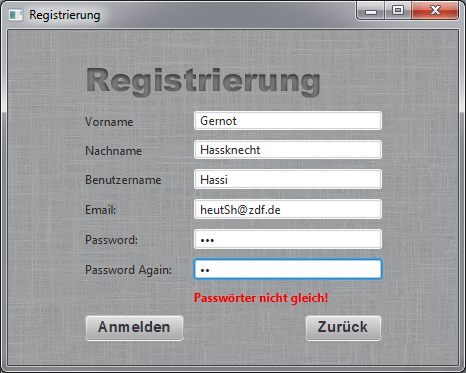
\includegraphics[scale=0.6]{regStage.png}
  		  \caption{Registrierung Fenster}
     \label{fig.RegistrierungFenster}
  \end{center}
\end{figure}

\subsection{Control}
\label{subsec.control}

Im Fenster \texttt{Control} ist es möglich, das Live-Video von der Cam zu betrachten. Es wird mit Hilfe der Klasse WebEngine und WebView realisiert. D.h. es wird durch WebEngine die Webseite geladen und durch WebView wird die geladene Webseite im Fenster angezeigt. Diese Webseite wird vom MJPEG Streamer zur Verfügung gestellt. Der Stream wird erst gestartet, wenn das Fenster \texttt{Control} geöffnet ist.

\begin{lstlisting}[caption={Stream Einbindung}\label{lst:reg.java.stream},captionpos=b]
WebView webview = new WebView();
webview.setVisible(true);
WebEngine webengine = webview.getEngine();
webengine.setJavaScriptEnabled(true);
File file = new File("http://<IP-Adresse vom PI>/javascript\_simple.html");
webengine.load(file.toString());
\end{lstlisting}

Beim Betätigen des Buttons \texttt{Database} wird ein neues Fenster \texttt{Datenbank} geöffnet (siehe Kapital \ref{subsec.datenbank}) und das Fenster \texttt{Control} wird geschlossen. 
Nach dem Betätigen des Buttons \texttt{Open} werden zwei Funktionen aufgerufen. Bei der ersten Funktion wird mit einem HTTP-POST ein Befehl an das PI gesendet, das dieses die Tür öffnen kann. Bei der zweiten Funktion wird ein neuer Eintrag in die Tabelle \texttt{tb\_doorloogers} in Datenbank eingetragen. Dieser Eintrag beinhaltet den Zeitpunkt des Öffnens der Tür.


\begin{figure}[h]
  \begin{center}
    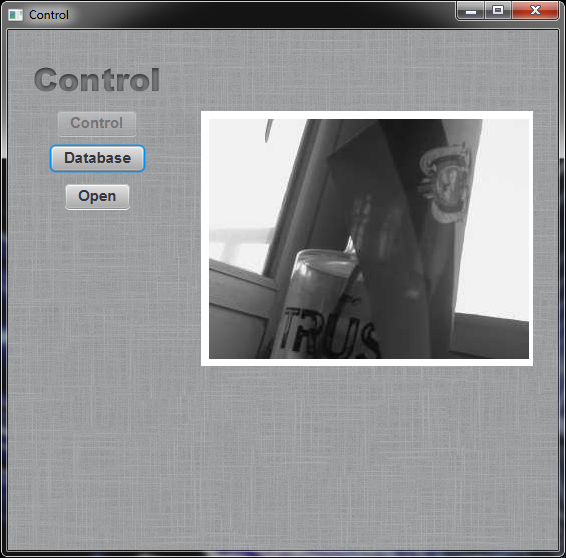
\includegraphics[scale=0.5]{streamStage.png}
  		  \caption{Control Fenster}
     \label{fig.StreamFenster}
  \end{center}
\end{figure}

\subsection{Datenbank}
\label{subsec.datenbank}
Diese Stage hat als Hauptobjekt eine Tabelle. Der Tabelleninhalt wird dynamisch erstellt. In einer zusätzliche Klasse wird geschaut, wie viele Spalten die Datenbank hat und fügt diese dann dem Tabellen-Objekt hinzu. Nach dem Hinzufügen der Spalten wird Zeile für Zeile aus der Datenbank geholt und in die Tabelle geladen. Zu jedem Eintrag in die Datenbanktabelle \texttt{tb\_doorlogger} gehört ein Bild. Um sich zu einen entsprechenden Tabelleneintrag das Bild anzusehen, muss man über eine Combobox die ID der Zeile auswählen und auf den Button \texttt{Open Picture} klicken. Mehr dazu im Kapitel \ref{subsec.foto}. Die Combobox zeigt nur so viele Zahlen wie es Zeilen in der Tabelle gibt. Wenn nichts in der Datenbank steht und dadurch auch kein Eintrag in die Tabelle gemacht wird, werden die Combobox und der \texttt{Open Picture} Button deaktiviert. Gibt es Einträge in der Datenbank, so ist die Standarteinstellung der Combobox auf 1.

\begin{figure}[h]
  \begin{center}
    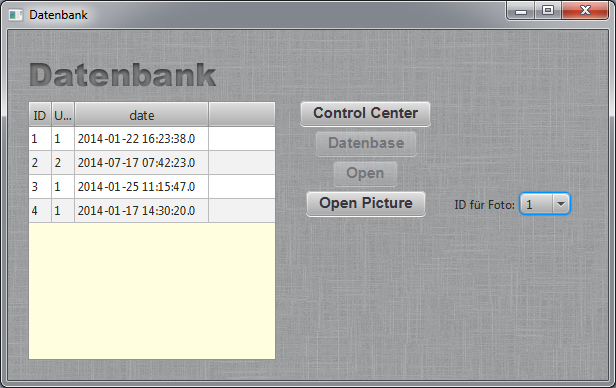
\includegraphics[scale=0.6]{dbStage.png}
  		  \caption{Datenbank Fenster}
     \label{fig.DatenbankFenster}
  \end{center}
\end{figure}

\subsection{Foto}
\label{subsec.foto}
Nachdem der \texttt{Open Picture} Button in der Datenbank Ansicht gedruckt wurde, wird mit Hilfe der angegebenen ID aus der Combobox der SQL-String gebaut.

\begin{lstlisting}[caption={Java-SQL String Foto öffnen}\label{lst:pic.db.foto.open},captionpos=b]
String SQL = "SELECT * FROM tb_images WHERE ID = " + userID;
\end{lstlisting}

Aus dem String ist relativ leicht zu erkennen, dass das Bild aus der Datenbanktabelle \texttt{tb\_images} kommt. Das Bild ist aber in der Datenbank nur binär als BLOB Typ abgelegt. Dieser Typ existiert auch in Java. Nach dem Auslesen des Binärstreams wandeln wir das Gelesene in ein Byte-Array. Aus dem Byte-Array erzeugen wir dann ein Buffered-Image. In Swing könnten wir uns jetzt schon ein Bild anzeigen lassen. Aber das Programm wurde ja nicht mit Swing, sondern mit JavaFX geschrieben. Dank eines \texttt{.toFXImage(BufferedImage arg0, WritableImage arg1)} Befehles lässt sich unser Swing-Objekt einfach in ein JavaFX-Objekt umwandeln. Dieses zeigen wir dann in einem zusätzlichen Stage Fenster an. Ein klarer Vorteil bei dieser Methode ist, dass es nicht wichtig ist, was für ein Typ dem Bild mal angehörte.
\begin{lstlisting}[caption={JavaFX Foto öffnen}\label{lst:pic.javafx.open},captionpos=b]
//Foto aus DB holen
byte[] imgData = imgShow.getImageDB(userID);
...
//Foto nach JavaFX Objekt wandeln
SwingFXUtils.toFXImage(bufImg, img2);

//Foto imageView hinzufügen
imageView.setImage(img2);
\end{lstlisting}

\section{Problematik der Verwaltung der Fenster}
Während der Entwicklung der Desktop Applikation in JavaFX gab es technische Schwierigkeiten mit der Schließung der einzelnen Fenster. Wenn im Fenster ein Button betätigt wird, der gleichzeitig ein neues Fenster öffnen und das aktuelle Fenster schließen soll, wird ungewollt der gesamte Java-Applikation Prozess gekillt. Besonders bei dem Fenster mit dem Stream gab es ein weiteres Problem, dass nach der Schließung des Stream-Fensters der Stream im Hintergrund weiterlief. Es muss ein Konzept zur korrekten Schließung der Fenster erstellt werden, sodass eine Window-Klasse die einzelnen Fenster zur Öffnung und Schließung steuert. Das Konzept wurde zum Teil aus Zeitgründen nicht vollständig umgesetzt. Die Umsetzung wurde jetzt so realisiert, dass das aktuelle Fenster zuerst das kommende Fenster aufruft, dann wird erst das aktuelle Fenster geschlossen. Bei dem Fenster mit dem Stream wurde nicht mit der Klasse \texttt{MediaView} sowie \texttt{MediaPlayer} gearbeitet, sondern mit der Klasse \texttt{webView} und \texttt{webEngine}. Damit konnte auch das Problem mit dem ungewollten Weiterlaufen des Streams im Hintergrund gelöst werden. %Desktop App
%%
%% Beuth Hochschule für Technik --  
%%
%% Kapitel 5 - Zusammenführung und Ausblick
%%
%%	

\chapter{Zusammenführung und Ausblick} %Zusammenführung und Ausblick

\listoffigures		%Abbildungsverzeichnis
\lstlistoflistings	%Listingverzeichnis
\begin{appendix}
  %%
%% Beuth Hochschule für Technik --  Abschlussarbeit
%%
%% Anhang
%%
%%%%%%%%%%%%%%%%%%%%%%%%%%%%%%%%%%%%%%%%%%%%%%%%%%%%%%%%%%%%%%%%%%%%%


\chapter{Anhang}



\end{appendix}
%%%%%%%%%%%%%%%%%%%%%%%%%%%%%%%%%%%%%%%%%%%%%%%%%%%%%%%%%%%%%%%
%% Literaturverzeichnis

\clearpage\newpage
\addcontentsline{toc}{chapter}{Literatur- und Quellenverzeichnis}
\bibliographystyle{IEEEtran}
\bibliography{bhtThesis}

\end{document}
